\documentclass[12pt]{article}
\usepackage{amsfonts}
\usepackage{amsmath}
\usepackage{amsthm}
\usepackage{graphicx}
\usepackage{fancyhdr}

\renewcommand{\headrulewidth}{0.4pt}

\addtolength{\oddsidemargin}{-.875in}
\addtolength{\evensidemargin}{-.875in}
\addtolength{\textwidth}{1.75in}
\addtolength{\topmargin}{-.875in}
\addtolength{\textheight}{1.75in}

\begin{document}
\title{Progress Report: (Week of July 10)}
\author{Samuel Wong}
\date{July 10, 2018}
\maketitle


\section{Samuel's Accomplished Tasks}
\subsection{Fixed a Bug of Changing Point Value in Gradient}
I discovered, with Mathew, that the gradient function I wrote in the beginning has a small bug. It accidentally adds $10^{-8}$ to each component of the given point each time it is called. We fixed this mistake.
\subsection{Confirmed Main Program Nan Come from Zero Gradient}
After fixing this mistake, we printed out the gradient of density whenever the main program returns "Nan". We found that every time the gradient is $[0,0,0,0,0,0]$. This is caused by us trying to normalize the vector. This test is good since it shows us that "Nan" do not come from any suspicious source of bug in the code.
\subsection{Wrote Sample Location for Mock Data}
I wrote a function that takes a density function as well as region in physical space desired for samples and it samples stars. It uses brute force accept-reject method. It seems to work quite fast on an explicit density function. But for qdf, it seems to be doing 0.13 second per star. This function should also handle the Toomre density function Mathew is working on.
\newpage
\subsection{Tested qdf Sample V on Set}
It seems that the KS statistics I have been using to test qdf sample V is not very good. It varies too much and depends too much on the number of points. So I decided to use another testing method, plotting the result using coloured scatter plot. The color represents vT that I sampled. I plotted sampled velocity using original function as well as the sampled velocity using my qdf sample v on set. I plotted them over each other (with dot size and shape different) and look for how well the two kinds of dots blend together through color. It seems to be working well.
\begin{figure}
  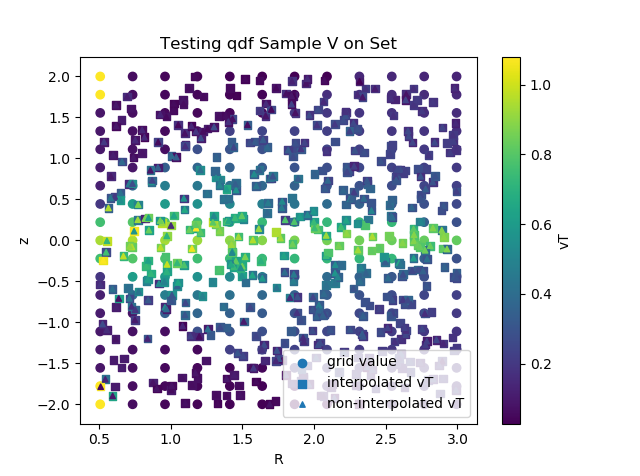
\includegraphics{sample v on set vs usual.png}
  \caption{Sample V on Set Testing.}
  \label{fig:sampleV}
\end{figure}

\newpage
\subsection{Derived and Implemented Analytic Energy and Momentum Gradient}
We have previously calculated $\nabla E$ and $\nabla L_z$ using numerical derivatives. We can do it better by finding the analytic expression for more accuracy.

First step is to write down the unit vector conversion between cylindrical coordinate and Cartesian coordinate since we work in Cartesian and the galpy potential is in cylindrical.
$$ \hat{R} = \cos(\phi) \hat{x} + \sin(\phi) \hat{y} $$
$$ \hat{\phi} = - \sin(\phi) \hat{x} + \cos(\phi) \hat{y} $$

\subsubsection{Deriving $\nabla L_z$}
The angular momentum per mass in z direction, written as a function of the 6 phase space coordinate, is given by
$$ L_z(x,y,z,v_x,v_y,v_z) = Rv_T $$
where $v_T$ is the tangential velocity in polar coordinate.

To put it more explicitly, since
$$ \phi = \arctan \left( \frac{y}{x} \right) $$
we have
\begin{align*}
\frac{d \phi}{dt} &= \frac{\partial}{\partial x} \left[ \arctan \left( \frac{y}{x} \right) \right] \frac{dx}{dt} + \frac{\partial}{\partial y} \left[ \arctan \left( \frac{y}{x} \right) \right] \frac{dy}{dt} \\
&= \frac{1}{1 + (y/x)^2} (y) (-x^{-2}) v_x + \frac{1}{1 + (y/x)^2} (\frac{1}{x}) v_y \\
&= \left( \frac{1}{1 + (y/x)^2} \right) \left[ \frac{-yv_x}{x^2}+\frac{v_y}{x}
  \right] \\
&= \left( \frac{x^2}{x^2 + y^2} \right) \left[ \frac{-yv_x + xv_y}{x^2} \right] \\
\frac{d \phi}{dt} &= \frac{xv_y - yv_x}{R^2}
\end{align*}

Since $v_T = R\dfrac{d \phi}{dt}$ and $L_z = Rv_T$, we have
$$ L_z = R^2\frac{d \phi}{dt} $$
Substituting,
$$ L_z = xv_y - yv_x $$

Taking the gradient in Cartesian,
$$ \nabla L_z = \frac{\partial L_z}{\partial x} \hat{x} + \frac{\partial L_z}{\partial y} \hat{y} +\frac{\partial L_z}{\partial z} \hat{z} + \frac{\partial L_z}{\partial v_x} \hat{v_x} + \frac{\partial L_z}{\partial v_y} \hat{v_y} + \frac{\partial L_z}{\partial v_z} \hat{v_z} $$
$$ \nabla L_z = v_y \hat{x} - v_x \hat{y} -y \hat{v_x} + x \hat{v_y} $$

In vector component form,
$$ \nabla L_z = [v_y, - v_x , 0, -y, x, 0] $$

\subsubsection{Deriving $\nabla E$}
The energy per mass is given by 
\begin{align*}
E(x,y,z,v_x,v_y,v_z) &= K(v_x,v_y,v_z) + \Phi(x,y,z) \\
&= \frac{1}{2}(v_x^2 + v_y^2 + v_z^2) + \Phi(x,y,z)
\end{align*}
Since $K$ does not depend on position,
\begin{align*}
\nabla K &= \frac{1}{2}(\frac{\partial v_x^2}{\partial v_x} \hat{v_x} +\frac{\partial v_y^2}{\partial v_y}\hat{v_y} + \frac{\partial v_z^2}{\partial v_z} \hat{v_z}) \\
&= v_x \hat{v_x} + v_y \hat{v_y} + v_z \hat{v_z} 
\end{align*}
The gradient of potential energy is negative force. Since galpy already implements this in cylindrical coordinate, we take the cylindrical gradient here. Since the potential is independent of velocity, our gradient only concerns the position.
\begin{align*}
 \nabla \Phi &= \hat{R} \frac{\partial \Phi}{\partial R} + \hat{\Phi} \frac{1}{R}\frac{\partial \Phi}{\partial \phi} + \hat{z}\frac{\partial \Phi}{\partial z} \\
&= - F_R \hat{R}  -F_{\phi} \hat{\Phi} - F_z \hat{z}
\end{align*}
Substituting the polar coordinate unit vector conversion to Cartesian,
\begin{align*}
 \nabla \Phi &= - F_R (\cos(\phi) \hat{x} + \sin(\phi) \hat{y})  -F_{\phi} (- \sin(\phi) \hat{x} + \cos(\phi) \hat{y}) - F_z \hat{z} \\
 &= \hat{x}(F_{\phi} \sin(\phi)- F_R \cos(\phi)) + \hat{y}(- F_R \sin(\phi) -F_{\phi} \cos(\phi)) - F_z \hat{z} \\
\end{align*}

Therefore, the gradient of energy is
$$ \nabla E =  \hat{x}(F_{\phi} \sin(\phi)- F_R \cos(\phi)) + \hat{y}(- F_R \sin(\phi) -F_{\phi} \cos(\phi)) - F_z \hat{z} + v_x \hat{v_x} + v_y \hat{v_y} + v_z \hat{v_z} $$

In vector component form, 
$$ \nabla E = [F_{\phi} \sin(\phi)- F_R \cos(\phi),- F_R \sin(\phi) -F_{\phi} \cos(\phi), - F_z ,v_x, v_y, v_z ] $$

\subsubsection{Testing and Comparison with Numerical Derivative}
I tested the analytic gradient function against numeric ones. The following is the printout of a test at a point:
\begin{align*}
\text{numeric} \nabla E &=  [0.05817276, 0.03358608, 0.13689572, 0.57735027, 0.57735027, 0.57735027]\\
\text{analytic} \nabla E &= [0.05817278, 0.03358607, 0.13689572, 0.57735027, 0.57735027, 0.57735027]
\end{align*}
\begin{align*}
 \text{numeric} \nabla L_z &=  [ 0.57735026, -0.57735027,  0.,         -1.00000001,  1.73205082,  0.        ] \\
 \text{analytic} \nabla L_z &= [ 0.57735027, -0.57735027,  0.,         -1.,          1.73205081,  0.        ] 
\end{align*}
This shows that both my derivation and the numerical gradient are correct, which in turns is the same gradient function we are using for density. So this adds more confidence in the main program.

\subsection{New Proposal for Checking Uniformity of Density}
I came up with a new way of checking the uniformity of density. Suppose there is  no $I_3$. Then we found the orthogonal complement of $\nabla E$ and $\nabla L_z$. Next we check whether $\nabla \rho$ is perpendicular to that complement. Since orthogonal complement of orthogonal complement is the original space, what we really want to check is whether $\nabla \rho$ is in the span of $\nabla E$ and $\nabla L_z$.

One way to check this is using the projection. We first use Gram-Schmidt to find orthonormal basis for $\nabla E$ and $\nabla L_z$. Let's call the two orthonormal vectors $\vec{v_1}$ and $\vec{v_2}$. If $\nabla \rho$ is in the span of $\vec{v_1}$ and $\vec{v_2}$, then $$\nabla \rho = (\nabla \rho \cdot \vec{v_1}) \vec{v_1} + (\nabla \rho \cdot \vec{v_2}) \vec{v_2} $$

Since this is never going to be exact, we can define the vector
$$ \vec{u} = (\nabla \rho \cdot \vec{v_1}) \vec{v_1} + (\nabla \rho \cdot \vec{v_2}) \vec{v_2} $$

Then we check how close this is to the original $\nabla \rho$. If we are going with the normalizing idea, we can normalize both and take their dot product:
$$ |\hat{\nabla \rho}| \cdot |\hat{u}| $$
Another method, proposed by Mathew, is that we can take the fractional length:
$$ \frac{|\vec{u}|}{|\nabla \rho|} $$

\section{Ayush’s Accomplished Tasks}


\section{Michael's Accomplished Tasks}


\section{Mathew's Accomplished Tasks}


\end{document}